\documentclass{prova}

\usepackage[portuguese]{babel}
\usepackage{amsmath}

\newcommand{\sen}{\mbox{sen}\,}
\newcommand{\ds}{\displaystyle}

\professor{Prof.\@ Adriano Barbosa}
\disciplina{C\'alculo Diferencial e Integral III}
\avaliacao{P2}
\curso{Engenharia Mec\^anica}
\data{13/06/2019}

\begin{document}
	\cabecalho{5}  % o numero 5 indica a qnt de quadros na tabela de nota

	\textbf{Todas as respostas devem ser justificadas.}
    \vspace{1cm}

	\begin{questionario}
        \q{Calcule a integral dupla $\ds\iint_D \sen{(x^2)}\ dA$, onde $D$ \'e a
        regi\~ao da figura 1.}
        \q{Calcule a integral dupla $\ds\int_{-3}^3\int_0^{\sqrt{9-x^2}}
        \sen{(x^2+y^2)}\ dy\ dx$.}
        \q{Sabendo que $\ds\iiint_E\ dV$ calcula o volume do s\'olido $E$,
        calcule o volume do s\'olido na figura 2.}
        \q{Calcule o trabalho realizado pelo campo $F(x,y,z) = (yz, xz, xy+2z)$
        ao mover uma part\'{\i}cula de $(0,0,0)$ a $(2,1,0)$.}
        \q{Use o Teorema de Green para calcular o trabalho realizado pelo campo
        $F(x,y) = (x(x+y), xy)$ ao mover uma part\'{\i}cula ao longo dos segmentos
        de reta de $(0,0)$ a $(1,0)$, de $(1,0)$ a $(0,1)$ e de $(0,1)$ a
        $(0,0)$.}
        \begin{figure}[h]
            \centering
            \begin{minipage}[h]{0.4\textwidth}
                \includegraphics[width=\textwidth]{q1.png}
                \caption{Exerc\'{\i}cio 1}
            \end{minipage}
            \hfill
            \begin{minipage}[h]{0.4\textwidth}
                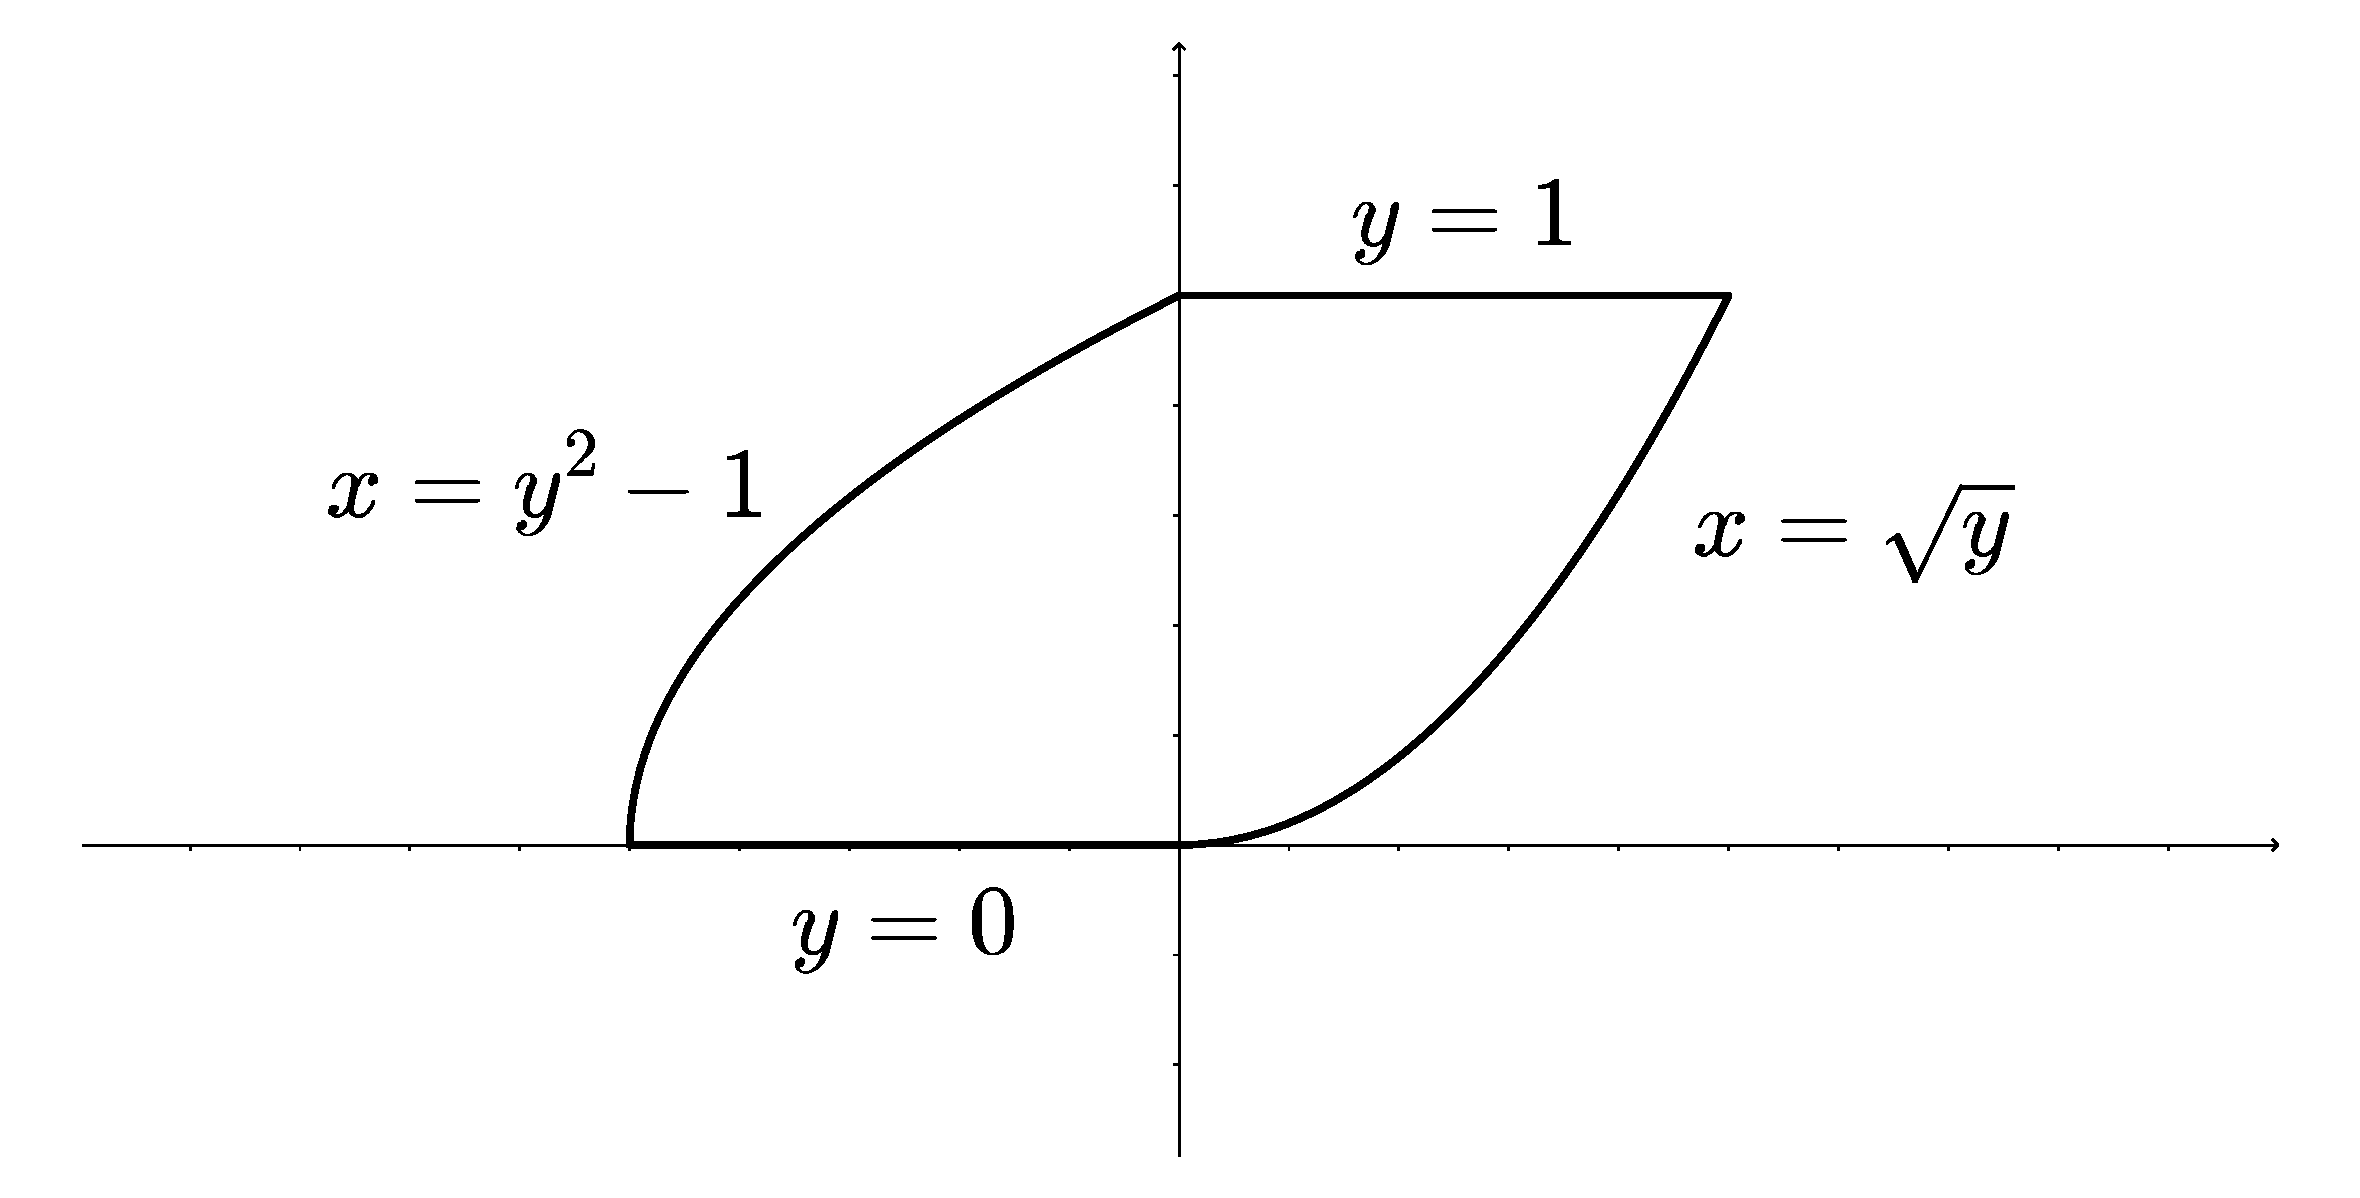
\includegraphics[width=\textwidth]{q3.png}
                \caption{Exerc\'{\i}cio 3}
            \end{minipage}
        \end{figure}
	\end{questionario}
\end{document}
